% RecSys Challenge 2026 Workshop Paper
% Multi-Stage Retrieval with Diverse Bi-Encoders for Conversational Music Recommendation
\documentclass[sigconf]{acmart}

% Remove default ACM copyright for submission
\setcopyright{none}
\settopmatter{printacmref=false}
\renewcommand\footnotetextcopyrightpermission[1]{}
\pagestyle{plain}

\usepackage{tikz}
\usetikzlibrary{positioning, fit, backgrounds}

\begin{document}

\title{Multi-Stage Retrieval with Diverse Bi-Encoders for\\Conversational Music Recommendation}

\author{Shuai Huang}
\affiliation{%
  \institution{University of North Carolina at Chapel Hill}
  \city{Chapel Hill}
  \state{NC}
  \country{USA}
}
\email{shuaishu@email.unc.edu}

\begin{abstract}
We present our solution to the RecSys Challenge 2026 on Conversational Music Recommendation (Music-CRS). The task requires recommending music tracks from a catalog of 47,071 items given multi-turn dialogue context and user profiles. Our approach employs a multi-stage pipeline: (1) diverse retrieval using multiple independently-trained bi-encoders (BGE, E5, NV-Embed-v2) alongside BM25 and collaborative filtering legs to maximize recall, (2) learned-to-rank fusion via LightGBM LambdaRank that exploits per-candidate features including raw cosine similarities, and (3) LLM-based response generation for natural language explanations. Key findings include: domain-fine-tuned bi-encoders with different base architectures provide complementary recall (+9.4\% nDCG@20 each), the 7.8B NV-Embed-v2 model provides unique recall that smaller models cannot match, and simple gradient-boosted reranking outperforms both pointwise and listwise neural rerankers on this task. Our system achieves nDCG@20 = 0.185 on the development set, a 127\% improvement over the official BM25 + LLaMA-1B baseline (0.0815). On the official Blind-B test set, our system obtains nDCG@20 = 0.304 with a composite score of 0.252 (rank 38/40). Code: \url{https://github.com/shuaih777/music-crs-challenge}. Team: shuaih.
\end{abstract}

\maketitle

\section{Introduction}

Conversational music recommendation systems aim to provide personalized music suggestions through natural language interactions, enabling users to iteratively refine their preferences across multiple dialogue turns. The RecSys Challenge 2026~\cite{recsys2026} introduces a conversational music recommendation task over 47,071 tracks, where systems must output a ranked list of 20 tracks and a natural language response at each turn. We participate as team \textbf{shuaih}.

This task presents two core challenges: (1) \textbf{recall}---finding the correct track among 47K candidates given only conversation context, and (2) \textbf{ranking precision}---ordering candidates correctly when the top-20 all share similar genres and attributes.

Our approach prioritizes recall expansion through model diversity. Rather than relying on a single retrieval model, we train multiple bi-encoders with different architectures (BGE-large, E5-large, NV-Embed-v2) on conversation-to-track matching, then fuse their candidates via learned-to-rank. This ``diverse retrieval + learned fusion'' paradigm consistently outperformed sophisticated neural reranking approaches in our experiments.

\section{System Architecture}

Our pipeline consists of three stages (Figure~\ref{fig:pipeline}):

% Pipeline figure for Music-CRS paper
% Compile standalone or include in main.tex with % Pipeline figure for Music-CRS paper
% Compile standalone or include in main.tex with % Pipeline figure for Music-CRS paper
% Compile standalone or include in main.tex with \input{fig_pipeline.tex}
% Requires: \usepackage{tikz} \usetikzlibrary{positioning, fit, backgrounds}
\begin{figure*}[t]
\centering
\resizebox{\textwidth}{!}{%
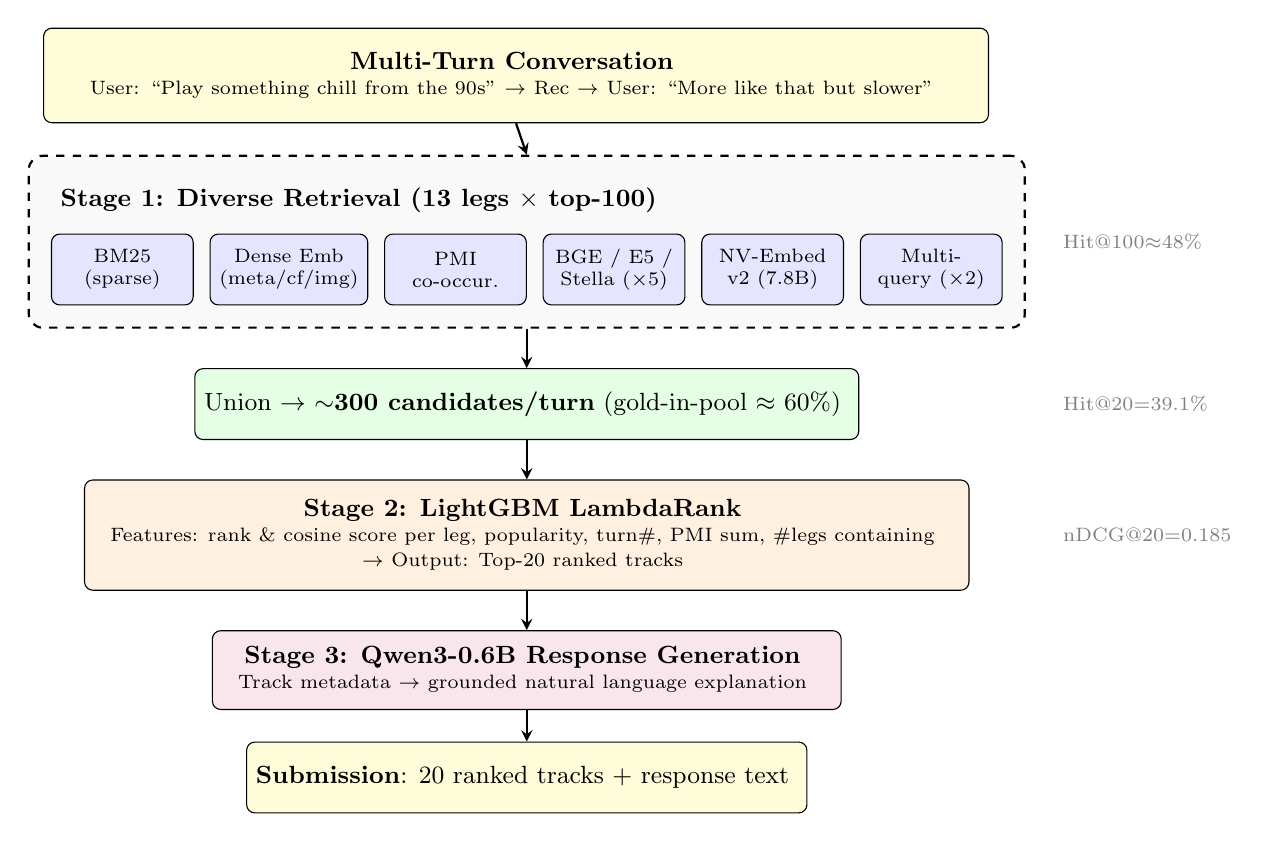
\begin{tikzpicture}[
    node distance=0.4cm and 0.3cm,
    box/.style={draw, rounded corners=3pt, align=center, minimum height=0.9cm, font=\small},
    stage/.style={draw, rounded corners=5pt, dashed, inner sep=8pt, thick, fill=gray!5},
    leg/.style={box, fill=blue!10, minimum width=1.8cm, font=\scriptsize},
    note/.style={font=\scriptsize, text=gray, anchor=west},
    arrow/.style={->, thick, >=stealth},
]

% Input
\node[box, fill=yellow!15, minimum width=12cm, minimum height=1.2cm] (input) {
    \begin{tabular}{c}
    \textbf{Multi-Turn Conversation} \\[-2pt]
    {\scriptsize User: ``Play something chill from the 90s'' $\to$ Rec $\to$ User: ``More like that but slower''}
    \end{tabular}
};

% Stage 1: retrieval legs
\node[leg, below=1.4cm of input, xshift=-5cm] (bm25) {BM25\\(sparse)};
\node[leg, right=0.2cm of bm25] (dense) {Dense Emb\\(meta/cf/img)};
\node[leg, right=0.2cm of dense] (pmi) {PMI\\co-occur.};
\node[leg, right=0.2cm of pmi] (bienc) {BGE / E5 /\\Stella ($\times$5)};
\node[leg, right=0.2cm of bienc] (nvemb) {NV-Embed\\v2 (7.8B)};
\node[leg, right=0.2cm of nvemb] (mq) {Multi-\\query ($\times$2)};

% Stage 1 title sits INSIDE the dashed box, so the incoming arrow (which stops
% at the box border) cannot run through it.
\node[font=\small\bfseries, anchor=south west] (s1title)
    at ([yshift=4pt]bm25.north west) {Stage 1: Diverse Retrieval (13 legs $\times$ top-100)};

\begin{scope}[on background layer]
\node[stage, fit=(s1title)(bm25)(dense)(pmi)(bienc)(nvemb)(mq)] (s1box) {};
\end{scope}

% Arrow from input to stage 1
\draw[arrow] (input.south) -- (s1box.north);

% Union node
\node[box, below=0.5cm of s1box, fill=green!10, minimum width=5cm] (union) {
    Union $\to$ \textbf{$\sim$300 candidates/turn} (gold-in-pool $\approx$ 60\%)
};
\draw[arrow] (s1box.south) -- (union.north);

% Stage 2
\node[box, below=0.5cm of union, fill=orange!12, minimum width=9cm, minimum height=1.4cm] (lgbm) {
    \begin{tabular}{c}
    \textbf{Stage 2: LightGBM LambdaRank} \\[-2pt]
    {\scriptsize Features: rank \& cosine score per leg, popularity, turn\#, PMI sum, \#legs containing}\\[-2pt]
    {\scriptsize $\to$ Output: Top-20 ranked tracks}
    \end{tabular}
};
\draw[arrow] (union.south) -- (lgbm.north);

% Stage 3
\node[box, below=0.5cm of lgbm, fill=purple!10, minimum width=7cm, minimum height=1cm] (resp) {
    \begin{tabular}{c}
    \textbf{Stage 3: Qwen3-0.6B Response Generation} \\[-2pt]
    {\scriptsize Track metadata $\to$ grounded natural language explanation}
    \end{tabular}
};
\draw[arrow] (lgbm.south) -- (resp.north);

% Output
\node[box, below=0.4cm of resp, fill=yellow!15, minimum width=6cm] (output) {
    \textbf{Submission}: 20 ranked tracks + response text
};
\draw[arrow] (resp.south) -- (output.north);

% Annotations, left-aligned in a single column just outside the widest box
\coordinate (ann) at ([xshift=0.35cm]s1box.east);
\node[note] at (ann)          {Hit@100$\approx$48\%};
\node[note] at (ann |- union) {Hit@20=39.1\%};
\node[note] at (ann |- lgbm)  {nDCG@20=0.185};

\end{tikzpicture}
}
\caption{System architecture. Stage 1 employs 13 diverse retrieval legs with different model architectures and query formulations. Their union forms a candidate pool with $\sim$60\% gold-track coverage. Stage 2 applies LightGBM LambdaRank to re-rank candidates using per-leg features. Stage 3 generates metadata-grounded responses.}
\label{fig:pipeline}
\end{figure*}

% Requires: \usepackage{tikz} \usetikzlibrary{positioning, fit, backgrounds}
\begin{figure*}[t]
\centering
\resizebox{\textwidth}{!}{%
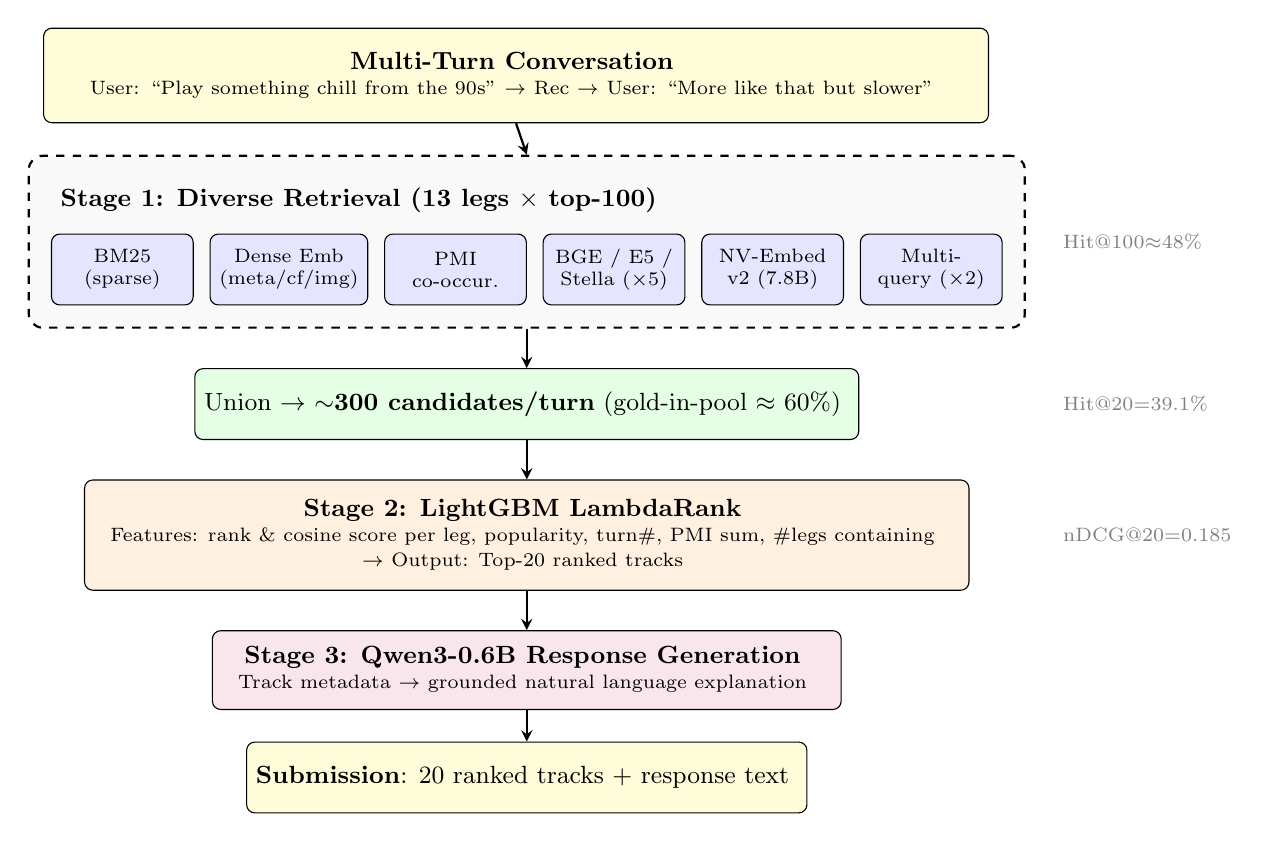
\begin{tikzpicture}[
    node distance=0.4cm and 0.3cm,
    box/.style={draw, rounded corners=3pt, align=center, minimum height=0.9cm, font=\small},
    stage/.style={draw, rounded corners=5pt, dashed, inner sep=8pt, thick, fill=gray!5},
    leg/.style={box, fill=blue!10, minimum width=1.8cm, font=\scriptsize},
    note/.style={font=\scriptsize, text=gray, anchor=west},
    arrow/.style={->, thick, >=stealth},
]

% Input
\node[box, fill=yellow!15, minimum width=12cm, minimum height=1.2cm] (input) {
    \begin{tabular}{c}
    \textbf{Multi-Turn Conversation} \\[-2pt]
    {\scriptsize User: ``Play something chill from the 90s'' $\to$ Rec $\to$ User: ``More like that but slower''}
    \end{tabular}
};

% Stage 1: retrieval legs
\node[leg, below=1.4cm of input, xshift=-5cm] (bm25) {BM25\\(sparse)};
\node[leg, right=0.2cm of bm25] (dense) {Dense Emb\\(meta/cf/img)};
\node[leg, right=0.2cm of dense] (pmi) {PMI\\co-occur.};
\node[leg, right=0.2cm of pmi] (bienc) {BGE / E5 /\\Stella ($\times$5)};
\node[leg, right=0.2cm of bienc] (nvemb) {NV-Embed\\v2 (7.8B)};
\node[leg, right=0.2cm of nvemb] (mq) {Multi-\\query ($\times$2)};

% Stage 1 title sits INSIDE the dashed box, so the incoming arrow (which stops
% at the box border) cannot run through it.
\node[font=\small\bfseries, anchor=south west] (s1title)
    at ([yshift=4pt]bm25.north west) {Stage 1: Diverse Retrieval (13 legs $\times$ top-100)};

\begin{scope}[on background layer]
\node[stage, fit=(s1title)(bm25)(dense)(pmi)(bienc)(nvemb)(mq)] (s1box) {};
\end{scope}

% Arrow from input to stage 1
\draw[arrow] (input.south) -- (s1box.north);

% Union node
\node[box, below=0.5cm of s1box, fill=green!10, minimum width=5cm] (union) {
    Union $\to$ \textbf{$\sim$300 candidates/turn} (gold-in-pool $\approx$ 60\%)
};
\draw[arrow] (s1box.south) -- (union.north);

% Stage 2
\node[box, below=0.5cm of union, fill=orange!12, minimum width=9cm, minimum height=1.4cm] (lgbm) {
    \begin{tabular}{c}
    \textbf{Stage 2: LightGBM LambdaRank} \\[-2pt]
    {\scriptsize Features: rank \& cosine score per leg, popularity, turn\#, PMI sum, \#legs containing}\\[-2pt]
    {\scriptsize $\to$ Output: Top-20 ranked tracks}
    \end{tabular}
};
\draw[arrow] (union.south) -- (lgbm.north);

% Stage 3
\node[box, below=0.5cm of lgbm, fill=purple!10, minimum width=7cm, minimum height=1cm] (resp) {
    \begin{tabular}{c}
    \textbf{Stage 3: Qwen3-0.6B Response Generation} \\[-2pt]
    {\scriptsize Track metadata $\to$ grounded natural language explanation}
    \end{tabular}
};
\draw[arrow] (lgbm.south) -- (resp.north);

% Output
\node[box, below=0.4cm of resp, fill=yellow!15, minimum width=6cm] (output) {
    \textbf{Submission}: 20 ranked tracks + response text
};
\draw[arrow] (resp.south) -- (output.north);

% Annotations, left-aligned in a single column just outside the widest box
\coordinate (ann) at ([xshift=0.35cm]s1box.east);
\node[note] at (ann)          {Hit@100$\approx$48\%};
\node[note] at (ann |- union) {Hit@20=39.1\%};
\node[note] at (ann |- lgbm)  {nDCG@20=0.185};

\end{tikzpicture}
}
\caption{System architecture. Stage 1 employs 13 diverse retrieval legs with different model architectures and query formulations. Their union forms a candidate pool with $\sim$60\% gold-track coverage. Stage 2 applies LightGBM LambdaRank to re-rank candidates using per-leg features. Stage 3 generates metadata-grounded responses.}
\label{fig:pipeline}
\end{figure*}

% Requires: \usepackage{tikz} \usetikzlibrary{positioning, fit, backgrounds}
\begin{figure*}[t]
\centering
\resizebox{\textwidth}{!}{%
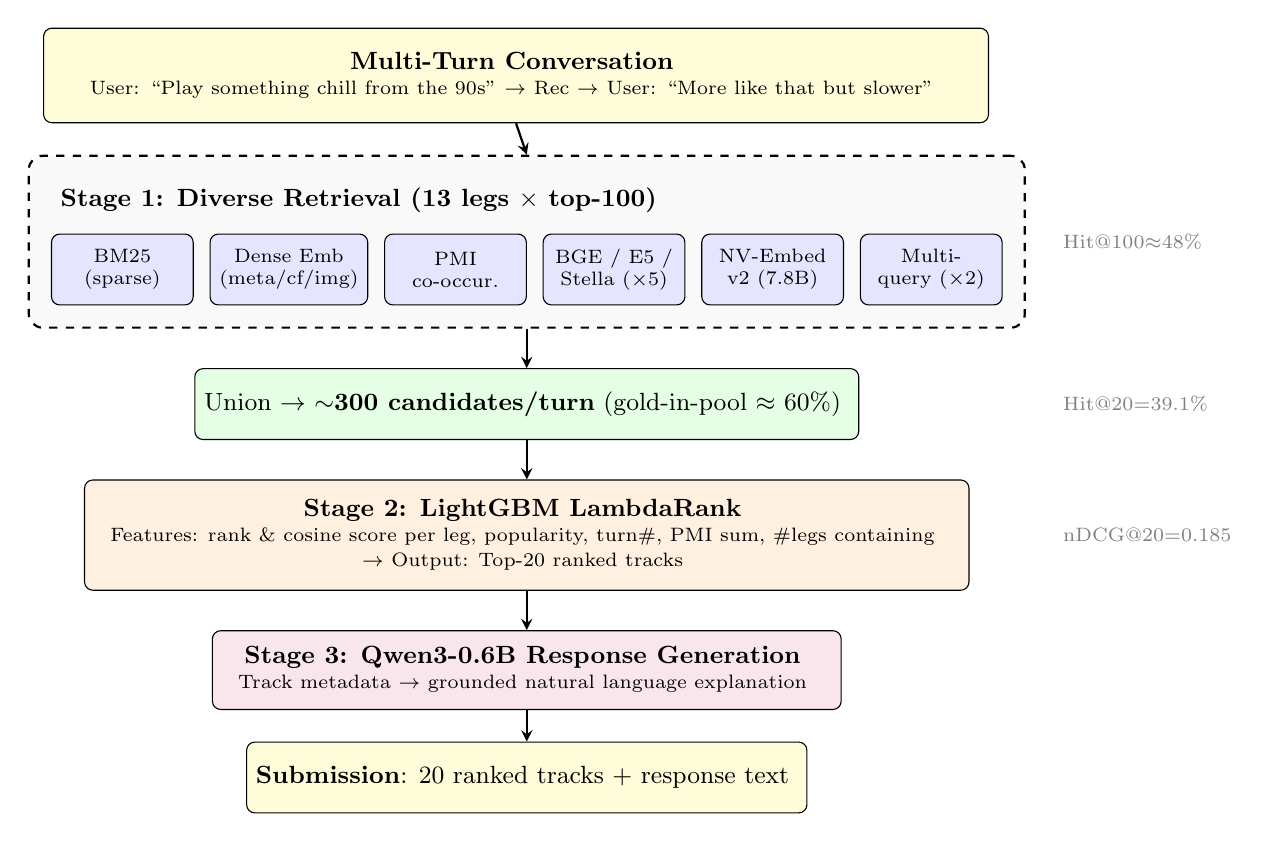
\begin{tikzpicture}[
    node distance=0.4cm and 0.3cm,
    box/.style={draw, rounded corners=3pt, align=center, minimum height=0.9cm, font=\small},
    stage/.style={draw, rounded corners=5pt, dashed, inner sep=8pt, thick, fill=gray!5},
    leg/.style={box, fill=blue!10, minimum width=1.8cm, font=\scriptsize},
    note/.style={font=\scriptsize, text=gray, anchor=west},
    arrow/.style={->, thick, >=stealth},
]

% Input
\node[box, fill=yellow!15, minimum width=12cm, minimum height=1.2cm] (input) {
    \begin{tabular}{c}
    \textbf{Multi-Turn Conversation} \\[-2pt]
    {\scriptsize User: ``Play something chill from the 90s'' $\to$ Rec $\to$ User: ``More like that but slower''}
    \end{tabular}
};

% Stage 1: retrieval legs
\node[leg, below=1.4cm of input, xshift=-5cm] (bm25) {BM25\\(sparse)};
\node[leg, right=0.2cm of bm25] (dense) {Dense Emb\\(meta/cf/img)};
\node[leg, right=0.2cm of dense] (pmi) {PMI\\co-occur.};
\node[leg, right=0.2cm of pmi] (bienc) {BGE / E5 /\\Stella ($\times$5)};
\node[leg, right=0.2cm of bienc] (nvemb) {NV-Embed\\v2 (7.8B)};
\node[leg, right=0.2cm of nvemb] (mq) {Multi-\\query ($\times$2)};

% Stage 1 title sits INSIDE the dashed box, so the incoming arrow (which stops
% at the box border) cannot run through it.
\node[font=\small\bfseries, anchor=south west] (s1title)
    at ([yshift=4pt]bm25.north west) {Stage 1: Diverse Retrieval (13 legs $\times$ top-100)};

\begin{scope}[on background layer]
\node[stage, fit=(s1title)(bm25)(dense)(pmi)(bienc)(nvemb)(mq)] (s1box) {};
\end{scope}

% Arrow from input to stage 1
\draw[arrow] (input.south) -- (s1box.north);

% Union node
\node[box, below=0.5cm of s1box, fill=green!10, minimum width=5cm] (union) {
    Union $\to$ \textbf{$\sim$300 candidates/turn} (gold-in-pool $\approx$ 60\%)
};
\draw[arrow] (s1box.south) -- (union.north);

% Stage 2
\node[box, below=0.5cm of union, fill=orange!12, minimum width=9cm, minimum height=1.4cm] (lgbm) {
    \begin{tabular}{c}
    \textbf{Stage 2: LightGBM LambdaRank} \\[-2pt]
    {\scriptsize Features: rank \& cosine score per leg, popularity, turn\#, PMI sum, \#legs containing}\\[-2pt]
    {\scriptsize $\to$ Output: Top-20 ranked tracks}
    \end{tabular}
};
\draw[arrow] (union.south) -- (lgbm.north);

% Stage 3
\node[box, below=0.5cm of lgbm, fill=purple!10, minimum width=7cm, minimum height=1cm] (resp) {
    \begin{tabular}{c}
    \textbf{Stage 3: Qwen3-0.6B Response Generation} \\[-2pt]
    {\scriptsize Track metadata $\to$ grounded natural language explanation}
    \end{tabular}
};
\draw[arrow] (lgbm.south) -- (resp.north);

% Output
\node[box, below=0.4cm of resp, fill=yellow!15, minimum width=6cm] (output) {
    \textbf{Submission}: 20 ranked tracks + response text
};
\draw[arrow] (resp.south) -- (output.north);

% Annotations, left-aligned in a single column just outside the widest box
\coordinate (ann) at ([xshift=0.35cm]s1box.east);
\node[note] at (ann)          {Hit@100$\approx$48\%};
\node[note] at (ann |- union) {Hit@20=39.1\%};
\node[note] at (ann |- lgbm)  {nDCG@20=0.185};

\end{tikzpicture}
}
\caption{System architecture. Stage 1 employs 13 diverse retrieval legs with different model architectures and query formulations. Their union forms a candidate pool with $\sim$60\% gold-track coverage. Stage 2 applies LightGBM LambdaRank to re-rank candidates using per-leg features. Stage 3 generates metadata-grounded responses.}
\label{fig:pipeline}
\end{figure*}


\subsection{Stage 1: Multi-Modal Retrieval}

We employ 13 independent retrieval legs, each producing a top-100 candidate list per (session, turn):

\textbf{Sparse retrieval.} BM25 over track metadata text (title, artist, album, tags, year) using conversation history as query.

\textbf{Dense retrieval (pre-computed embeddings).} Cosine similarity between mean-pooled embeddings of previously accepted tracks and all catalog tracks, using the dataset's pre-computed modality embeddings: metadata-qwen3 (1024d), CF-BPR (128d), and image-SigLIP2 (768d).

\textbf{Fine-tuned bi-encoders.} We train sentence-transformers bi-encoders on 120K (conversation, gold\_track) pairs with MultipleNegativesRankingLoss (in-batch negatives). We use five different base models: BGE-base-en-v1.5 (110M), BGE-large-en-v1.5 (335M), E5-large-v2 (335M), Stella-400M, and NV-Embed-v2 (7.8B). Each provides partially non-overlapping recall.

\textbf{Co-occurrence.} Session-level item-item PPMI computed from 15K training sessions.

\textbf{Multi-query variants.} The BGE-large encoder with alternative query formulations: last-2-turns only and current-utterance only.

\subsection{Stage 2: Learned-to-Rank Fusion}

We form a candidate pool by taking the union of all 13 legs' top-100 outputs ($\sim$200--400 unique candidates per turn). A LightGBM LambdaRank model is trained to re-rank candidates with the following features per candidate:

\begin{itemize}
    \item Rank and RRF-style score ($1/(60+\text{rank})$) in each leg
    \item Raw cosine similarity from the bi-encoder (continuous feature)
    \item Track popularity, turn number, number of prior accepts
    \item PMI sum with previously accepted tracks
    \item Number of legs containing this candidate
\end{itemize}

The model is trained with 5-fold grouped cross-validation on the development set, optimizing nDCG@20 directly.

\subsection{Stage 3: Response Generation}

We generate natural language responses using Qwen3-0.6B with metadata-grounded prompts. The model receives the recommended track's metadata (title, artist, genre tags, year) and produces a brief explanation. We use nucleus sampling (top-p=0.85, temperature=0.7) with repetition penalty to maximize lexical diversity (Distinct-2).

\section{Key Design Decisions}

\subsection{Model Diversity over Model Size}

Our most important finding is that \textbf{recall expansion through model diversity} dominates all other improvements. Table~\ref{tab:ablation} shows that each new bi-encoder with a different architecture adds +0.003--0.009 nDCG@20, while attempts to improve ranking within the existing candidate pool (cross-encoders, listwise rerankers) consistently failed.

\subsection{Why Neural Rerankers Failed}

We conducted extensive experiments with transformer-based rerankers:
\begin{itemize}
    \item Pointwise cross-encoder (Qwen3-0.6B, LoRA): $-0.5\%$ with random negatives, $-0.5\%$ with hard negatives
    \item Listwise reranker (Qwen3-8B, zero-shot): $-1.8\%$
    \item Fine-tuned listwise (Qwen3-1.5B, LoRA): $-0.6\%$ vs LightGBM
\end{itemize}

We hypothesize this occurs because the top-20 candidates from our retrieval stage all share highly similar metadata (same genre, era, mood), making them indistinguishable to language models that lack deep music-domain knowledge. The LightGBM ``voting'' feature (number of legs containing a candidate) provides a stronger signal than semantic understanding for this task.

\subsection{NV-Embed-v2 as Retrieval Backbone}

The single largest improvement came from NV-Embed-v2 (7.8B parameters), which contributed +0.011 nDCG@20 as a retrieval leg. Its superior encoding capacity captures nuanced conversation-to-track relationships that 335M models miss, providing unique recall on approximately 5\% of queries.

\section{Experiments}

\subsection{Dataset}

The TalkPlayData-Challenge dataset~\cite{talkplay2026} contains 15,199 training and 1,000 development sessions, each with 8 conversation turns. The track catalog has 47,071 items with metadata, tags, and pre-computed embeddings across 6 modalities. We use \textbf{no additional external datasets}; all training is conducted exclusively on the provided challenge data.

\subsection{Evaluation}

We report nDCG@\{1, 10, 20\}, Hit@20 (proportion of turns where the gold track appears in top-20), and Distinct-2 for response diversity. The official blind evaluation additionally uses Gemini LLM-as-judge for response quality.

\subsection{Results}

\begin{table}[h]
\centering
\caption{Development set results. Baseline is the official LLaMA-3.2-1B + BM25.}
\label{tab:results}
\small
\setlength{\tabcolsep}{4pt}
\begin{tabular}{@{}lcccc@{}}
\toprule
System & nDCG@20 & Hit@20 & nDCG@1 & Dist-2 \\
\midrule
Official baseline & 0.082 & -- & 0.010 & 0.255 \\
BM25 + no-repeat & 0.100 & 20.6\% & 0.036 & 0.090 \\
RRF (3 legs) & 0.128 & 26.7\% & 0.044 & 0.097 \\
LightGBM (9 legs) & 0.146 & 30.8\% & 0.051 & -- \\
+ BGE-base bi-enc & 0.156 & 33.5\% & 0.050 & -- \\
+ BGE-large bi-enc & 0.165 & 35.2\% & 0.052 & -- \\
+ NV-Embed-v2 & \textbf{0.185} & \textbf{39.1\%} & \textbf{0.064} & -- \\
+ Responses & 0.185 & 39.1\% & 0.064 & 0.261 \\
\bottomrule
\end{tabular}
\end{table}

\subsection{Ablation: Retrieval Legs}

\begin{table}[h]
\centering
\caption{Incremental contribution of each retrieval leg type.}
\label{tab:ablation}
\small
\setlength{\tabcolsep}{4pt}
\begin{tabular}{@{}lcc@{}}
\toprule
Addition & $\Delta$ nDCG@20 & Hit@20 \\
\midrule
BM25 + dense (baseline) & -- & 30.8\% \\
+ PMI co-occurrence & +0.004 & 26.7\% \\
+ BGE-base bi-encoder & +0.009 & 33.5\% \\
+ BGE-large bi-encoder & +0.009 & 35.2\% \\
+ E5-large bi-encoder & +0.003 & 35.8\% \\
+ Stella-400M & +0.003 & 38.3\% \\
+ NV-Embed-v2 (7.8B) & +0.011 & 39.1\% \\
\midrule
Pointwise cross-encoder & $-0.005$ & -- \\
Listwise reranker (8B) & $-0.003$ & -- \\
\bottomrule
\end{tabular}
\end{table}

\subsection{Per-Turn Analysis}

Performance varies significantly across turns: Turn 2 achieves the highest nDCG@20 (0.21) as the model has one prior accept as signal, while Turn 1 (explicit queries) and Turns 7--8 (conversation drift) are weakest. The collaborative filtering and bi-encoder legs are most valuable at later turns.

\subsection{Blind Test Set Results}

On the official Blind-B evaluation, our system achieves a composite score of 0.252 (nDCG@20 = 0.304, Catalog Diversity = 0.031, Lexical Diversity = 0.629, LLM-as-a-Judge = 1.45). While nDCG@20 improves significantly over our development set performance, the low Catalog Diversity score (0.031) indicates that our system over-concentrates recommendations on a small subset of popular tracks. This is a known limitation of the ``voting'' mechanism in our LightGBM reranker, which favors tracks appearing in multiple retrieval legs---these tend to be well-known items. A post-hoc diversification step (e.g., MMR) would likely address this but was not implemented before the deadline.

\section{Conclusion}

Our solution demonstrates that for conversational music recommendation with a large catalog, diverse retrieval ensembles with learned fusion substantially outperform neural reranking approaches. The key insight is that \textbf{recall is the binding constraint}: with 47K tracks, finding the correct item is harder than ranking it, and model diversity in the retrieval stage provides the largest gains. Future work could explore end-to-end generative approaches (semantic ID prediction) which bypass the retrieve-then-rerank paradigm entirely.

\begin{thebibliography}{9}

\bibitem{recsys2026}
S.~Doh, S.~Oramas, B.~Sguerra, A.~Bohra, C.~Pomo, F.~Barile.
\newblock RecSys Challenge 2026: Conversational Music Recommendation.
\newblock \url{https://www.recsyschallenge.com/2026/}

\bibitem{talkplay2026}
S.~Doh, K.~Choi, J.~Nam.
\newblock TalkPlay: Multimodal Music Recommendation with Large Language Models.
\newblock arXiv:2502.13713, 2026.

\bibitem{lightgbm}
G.~Ke, Q.~Meng, T.~Finley, et al.
\newblock LightGBM: A Highly Efficient Gradient Boosting Decision Tree.
\newblock NeurIPS, 2017.

\bibitem{bge}
S.~Xiao, Z.~Liu, P.~Zhang, N.~Muennighoff.
\newblock C-Pack: Packaged Resources to Advance General Chinese Embedding.
\newblock arXiv:2309.07597, 2023.

\bibitem{nvembed}
C.~Lee, R.~Roy, et al.
\newblock NV-Embed: Improved Techniques for Training LLMs as Generalist Embedding Models.
\newblock arXiv:2405.17428, 2024.

\bibitem{mnrl}
N.~Reimers, I.~Gurevych.
\newblock Sentence-BERT: Sentence Embeddings using Siamese BERT-Networks.
\newblock EMNLP, 2019.

\bibitem{gcrs}
S.~Zhang, M.~Liu, C.~Long.
\newblock Generative Conversational Recommender System.
\newblock arXiv:2605.21987, 2026.

\bibitem{e5}
L.~Wang, N.~Yang, X.~Huang, et al.
\newblock Text Embeddings by Weakly-Supervised Contrastive Pre-training.
\newblock arXiv:2212.03533, 2022.

\bibitem{lambdarank}
C.~Burges, R.~Ragno, Q.~Le.
\newblock Learning to Rank with Nonsmooth Cost Functions.
\newblock NeurIPS, 2006.

\end{thebibliography}

\end{document}
